% Author rewrite track. Body is empty; headings only until new text is inserted.
% Compile when asked: pdflatex main_rewrite.tex (twice).
% Bibliography: bibliography.tex (inserted at the end).
\documentclass[11pt,a4paper]{article}

\usepackage[margin=1in]{geometry}
\usepackage{times}
\renewcommand{\ttdefault}{cmtt}
\usepackage{amsmath,amssymb}
\usepackage{booktabs}
\usepackage{graphicx}
\usepackage{xcolor}
\usepackage{hyperref}
\usepackage[numbers,sort&compress]{natbib}
\usepackage{setspace}
\usepackage{caption}
\usepackage{float}
\usepackage{tabularx}

\hypersetup{colorlinks=true,linkcolor=blue,citecolor=blue,urlcolor=blue}
\setstretch{1.15}
\captionsetup{font=footnotesize,labelfont=bf,skip=6pt}

\title{\textbf{Plasma Protein Binding Prediction under Scaffold Split: Tree Models, ChemBERTa, Graph Networks, and Late Fusion}}

\author{%
  \begin{tabular}{c}
    Pradyumna Kumar Pradhan\textsuperscript{1}%
      \thanks{Corresponding author. Independent researcher.}\\[0.55em]
    \small\textsuperscript{1}Independent researcher\\[0.2em]
    \small Formerly, University of North Carolina at Greensboro\\
    \small (UNC Greensboro), Greensboro, NC, USA
  \end{tabular}%
}

\date{}
\graphicspath{{./}{../../figures/}}

\begin{document}
\maketitle

\begin{abstract}
\noindent
From idea generation to testing, drug discovery is a lengthy and expensive process.
Rather than chasing all of their molecule ideas, scientists prioritize certain molecules that are more likely to be successful, from synthesis to safety to therapeutic use.
Machine learning and AI enable researchers to narrow their candidate choices by predicting important properties such as ADMET (Absorption, Distribution, Metabolism, Excretion, and Toxicity).

This study uses the Plasma Protein Binding (PPB) dataset from DeepChem's MoleculeNet~\cite{wu2018moleculenet}, with several graph neural networks (GNNs), ChemBERTa (a language model for SMILES strings of molecules), and fusions of these models.
The performance of these neural models is compared against two standard tree-based models: Random Forest (RF) and XGBoost.
Instead of random splitting of the dataset, this study evaluates the models based on scaffold splitting that separates molecules by the Bemis--Murcko scaffold~\cite{bemis1996scaffold} and puts the entire group into only the training, validation, or testing set.

This study demonstrates that for the PPB dataset, GNNs and ChemBERTa models perform better than the tree models.
On a mean basis, the fusion models perform better than the individual GNNs or ChemBERTa-only models.
Random splitting on the RF model exhibits a better $R^{2}$ score than on a scaffold-split dataset.
Because under scaffold splitting the model predicts on unseen cores, the task becomes more difficult than under regular random splitting.

\vspace{0.4em}
\noindent\textbf{Keywords:} plasma protein binding, DeepChem, MoleculeNet, ChemBERTa, graph neural networks, scaffold split, late fusion
\end{abstract}

\section{Introduction}

Bringing a small-molecule drug to the market is a long and slow process that involves many iterations of structural design refinement and experimental validation.
During this development process, the chemists constantly evaluate the ADMET (Absorption, Distribution, Metabolism, Excretion, and Toxicity) properties of these molecules~\cite{bohnert2013ppb}.
How drugs are being absorbed, distributed, metabolized, or excreted from our system determines how much drug is available and therefore whether an effective exposure can be reached.
Scientists also use the ADMET properties to evaluate the dose amount and schedule.
Although these properties can be measured in the lab, it creates a significant logistical challenge.
Synthesizing a molecule and then testing it individually are resource-intensive processes.
Hence, the scientists must optimize the number of molecules they should prioritize synthesizing and testing in a physical laboratory by narrowing their choices through a computational approach.
Machine Learning (ML) and Deep Learning (DL) models have given the scientists a much-needed arsenal to speed up this process.

Plasma protein binding (PPB) is one such important endpoint that influences the ADMET properties of a molecule.
When a drug is absorbed or inserted into the plasma, a percentage of those molecules get attached to plasma proteins, primarily to albumin (more binding sites and binds to acidic molecules) and smaller portions to the alpha-1-acid glycoprotein (AAG) (fewer binding sites and binds to basic molecules) and lipoproteins.
Thus, PPB decreases the true available drug molecule in the solution state.
PPB is represented by the following ratio: number of molecules attached to the plasma proteins vs the total number of molecules in the plasma, both in solution state and bound state.

Binding to plasma proteins decreases the number of available molecules in the solution state.
Hence, PPB largely influences what percentage of the total injected drug will arrive at the target or be absorbed into the cell.
PPB can also influence the half-life of a drug inside the system: how quickly they are being metabolized or excreted out from the system.
Since many drug molecules bind to plasma proteins reversibly, and remain in an equilibrium state with their solution counterpart, plasma proteins sometimes serve as a mini-reservoir that releases drug slowly into the system thus increasing the half-life.

Different drug molecules bind to the plasma proteins with different affinity.
Because the binding is reversible, a drug molecule with higher affinity can replace a drug molecule with lower affinity.
For example, if drug A has lower affinity than drug B, the dose of drug A should be tightly controlled.
Because if both A and B are taken concurrently, the unbound drug A will be present in higher concentration in the system than the original intended amount.
Higher concentrations of free A can lead to toxicity~\cite{bohnert2013ppb}.
Thus, it is critical to know the PPB values for each drug, and PPB is an important property to predict.

DeepChem's sub-module MoleculeNet (MolNet) provides curated public datasets to evaluate many endpoint properties including PPB~\cite{wu2018moleculenet}.
These datasets can be loaded and compared in one place through many wrapper functions and ML/DL algorithms provided by DeepChem.
For benchmark reproducibility, DeepChem also provides many standard featurizers and splitters for these datasets.

Molecular featurization is one of the key challenges encountered by an ML engineer when they are trying to teach the structure of a molecule to a computer.
A molecule must be represented by a numerical vector that somehow encodes the structure and chemical property of that molecule, so that the machine will use it to predict the task assigned to it.
DeepChem offers many such wrapper algorithms, also called molecule featurization functions; examples include Graph Convolution Featurizers, RoBERTa Featurizer, RDKitGrid Featurizer, FASTA featurizer, etc.

The performance of a model hugely gets affected by the splitting technique.
DeepChem offers many splitter functions including random and scaffold splitters.
If someone wants to design a robust model, then random splitting of the dataset is not ideal.
If the testing dataset has molecules with a similar core to the training dataset samples, the model can use that shared core and hence the knowledge will not be transferable when it encounters a molecule with a different core.
Therefore, random splitting often elevates the metrics that are attributed more toward the splitting choice than the model itself.

A core/scaffold of a molecule is typically the ring systems and the atoms that join those rings, upon which a group of molecules are built by adding a variety of functional groups or atoms, thus creating different molecules~\cite{bemis1996scaffold}.
Splitting by these cores is called ``scaffold splitting,'' in which the molecules are separated based on their core/scaffold structures~\cite{wu2018moleculenet}.
The training set, evaluation set, and testing set all have different cores, thus the knowledge acquired by the model can be transferable when the model is applied to a different group of molecules with a different core.

The DeepChem package simplifies the benchmarking process by providing a one-stop shop for algorithms needed: splitting, loading, featurizing, training, and testing with metrics wrappers.
In 2009, ImageNet, which introduced benchmarking for image classification, played a big role in the development of modern AI, including convolutional neural networks.
DeepChem aims to provide similar support through their open-source module in building models to predict tasks in medicinal chemistry, quantum chemistry, biochemistry, and genomics.

This study uses the PPB dataset from DeepChem's MoleculeNet~\cite{wu2018moleculenet}.
The dataset offers 1614 molecules and their PPB values in percentage.
This study evaluates the performance of GCN~\cite{kipf2017gcn}, GIN~\cite{xu2019gin}, and GAT~\cite{velickovic2018gat} (three graph neural networks), ChemBERTa (a language model)~\cite{chithrananda2020chemberta}, and the following fusion models: ChemBERTa+GCN, ChemBERTa+GIN, ChemBERTa+GAT, and GCN+GIN+GAT.
For this evaluation, two simple tree models, Random Forest (RF) and XGBoost, on circular fingerprints (ECFP)~\cite{rogers2010ecfp}, are used as the baseline.
The dataset is split using one Bemis--Murcko scaffold split.
Models are tested using three seeds: 42, 43, and 44.
A split comparison between random and scaffold splitting techniques is also made using the Random Forest model.

\section{Methods}
\label{sec:methods}

\subsection{Data and labels}
This study uses the PPB dataset loaded from DeepChem's MoleculeNet~\cite{wu2018moleculenet,ramsundar2019deep}.
In the PPB dataset, the $y$-label represents the percent of the drug molecule bound to the plasma proteins.
The $y$-label was preprocessed using DeepChem's normalization transformer that applies $z$-score scaling.
$Z$-score is defined as $Y_{\mathrm{norm}} = (y - \mathrm{mean})/\mathrm{std}$, where $Y_{\mathrm{norm}}$ is the normalized $y$-label, $y$ is the true $y$-label, mean is the mean of the $y$-labels of the training set and std is the standard deviation of the $y$-labels of the training set.
Mean and std were calculated using only the training set and then applied to the validation and test sets, so that the scaling wouldn't be affected by the unseen test and validation sets.

\subsection{Splits and seeds}
During a drug discovery process, scientists often design molecules using a new molecular core/scaffold and often create a family of molecules by attaching different substituents to the core.
The cores are often a collection of ring structures connected by linker atoms or bonds.
This core is called the molecule's Murcko scaffold~\cite{bemis1996scaffold}.
When two molecules share the same scaffold irrespective of their substituents, they are grouped into the same scaffold label.
Essentially, the scaffold label serves as a chemical-family-lineage tag for that drug molecule.

This study used DeepChem's built-in scaffold splitter.
This splitter groups molecules with the same Bemis--Murcko scaffold via RDKit and then assigns the entire group into either the training, validation, or testing set.
A Bemis--Murcko scaffold may differ from a chemist-drawn core.
A model is only as good as its ability to predict relevant molecular properties for an unseen core/scaffold.
Scaffold splitting forces the model to predict on Murcko scaffolds that it has never seen before, though close analog scaffolds can still appear across splits.
Scaffold splitting is a much harder task for a model than training on a randomly split sample, in which molecules with similar structures and cores are divided into training, validation, and testing sets~\cite{wu2018moleculenet,sheridan2013time}.

All the models in this study were compared using one Bemis--Murcko scaffold split.
Post-split, the resulting sizes were 1291/161/162 (training/validation/testing) for the PPB dataset.
Every model was featurized, trained, and evaluated on the same set of molecules.

Random seeds 42, 43, and 44 were used throughout the process.
These seeds only affected weight initialization, dropout, data-order shuffling for all the models, and also the tree random states for the tree-only models; they did not affect the splitting.

As a control, a Random Forest (RF) model with Extended-Connectivity Fingerprints (ECFP)~\cite{rogers2010ecfp} was trained using the random splitter.
The control used the same random seeds, and same nominal training, validation, and testing sizes as the scaffold-split RF+ECFP run.
This control training demonstrates the relative ease of prediction when compounds with similar cores exist in the training, validation, and testing sets.

\subsection{Models and training protocol}

\subsubsection{Random Forest (RF) and Extreme Gradient Boosting (XGBoost)}
This study uses two decision-based tree models: Random Forest (RF) and XGBoost.
The RF creates an ensemble of decision trees from bootstrap samples of the training data.
The RF builds each of these decision trees based on a random group of features at each split.
This random group of features enables the model to generalize and reduces the risk of overfitting.
In a classification problem, the final decision is decided by majority vote.
In a regression problem, the final prediction is a mean of the predictions from all the trees.

XGBoost, on the other hand, builds decision trees sequentially.
Each new tree tries to correct the mistakes of the previous trees.
Correcting these mistakes reduces the errors in each step.
For both the classification problem and the regression problem, the sum of all the trees predicts the final value.
For the classification problem, this sum is then passed through a sigmoid (binary) or a softmax (multi-class).
For many ML benchmarking tasks, RF and XGBoost are often used as baselines.

Using DeepChem's ECFP featurization function, for all the SMILES in the PPB dataset, circular fingerprints were generated as 1024-bit vectors with radius 2~\cite{rogers2010ecfp}.
No hyperparameter tuning was run for either RF or XGBoost models.
The following basic parameters were used as a baseline for this study.
RF used 200 trees, whereas the XGBoost used 300 trees, with a maximum depth of 6 and a learning rate of 0.05.

\subsubsection{ChemBERTa language model}
This study uses ChemBERTa, a pretrained transformer language model that tries to understand the chemistry from SMILES strings~\cite{chithrananda2020chemberta}.
In SMILES notation, the molecules are written as a string of characters, for example the Aspirin molecule can be written as \texttt{CC(=O)Oc1ccccc1C(=O)O}.
ChemBERTa is a pre-trained BERT model that is an encoder-only variation of RoBERTa.
This variation of ChemBERTa that was downloaded from Hugging Face was trained on a corpus of 100k SMILES strings from the ZINC dataset.
In this study, a regression head is attached to the encoder stack of ChemBERTa for property prediction.

During the pre-training process of ChemBERTa, a SMILES string is split into tokens, and each token is converted into a vector of a given dimension called an embedding vector.
To this embedding vector, another vector that represents the position of that token is added.
This positional encoding is an important step as it provides the network with the information about the position of each token in that SMILES string.
Each encoder block uses a multi-head attention layer.
The output from the multi-head attention is added to the residual connection from the block input and then fed into a layer normalization layer, followed by a feed-forward network.
The output from the feed-forward network is again added to the residual connection from the post-multi-head attention layer and then fed into a layer normalization layer.
Several of these encoder blocks are stacked in the encoder.
During the training process, for the first two epochs the transformer model weights are frozen.
The model is trying to learn the regression task at hand by optimizing the weights of the regression head.
If the rest of the model parameters are not frozen during the early part of this training, changing the encoder weights may disrupt the semantics learned during the pre-training of ChemBERTa.

The ChemBERTa model was downloaded from Hugging Face: \texttt{seyonec/ChemBERTa-zinc-base-v1} with the matching tokenizer (\texttt{AutoTokenizer}).
Uncanonicalized SMILES strings directly from DeepChem's PPB dataset were used to tokenize.
Input token sequences were either truncated or padded to a maximum length of 128.
Each token is then converted into an embedding vector of dimension 768, also called the hidden state dimension.
A linear regression head was attached to the pooled [CLS] output of the encoder-only transformer architecture of the ChemBERTa model.
The regression model used in this study was \texttt{AutoModelForSequenceClassification} with \texttt{problem\_type='regression'} and \texttt{num\_labels=1}.
The training was completed using 20 epochs with a batch size of 32, AdamW optimizer at a learning rate of $1\times 10^{-5}$, and weight decay of 0.01.
At every step, the gradients were clipped at a maximum norm of 1.0.

During the first two epochs, all the encoder parameters, including the embeddings, were frozen and only the regression head's parameters were trained and updated.
On epoch three, all the layers were unfrozen and all the parameters were trained using a new AdamW optimizer with the same learning rate.
The model checkpoint with the highest validation $R^{2}$ value among all the epochs was saved and used to evaluate the testing samples.
The current learning rate and freezing schedule were chosen after an exploratory hyper-parameter-tuning experiment for the PPB dataset.

\subsubsection{Graph networks (GCN, GIN, GAT)}
\label{sec:graph-networks}
This study uses three different Graph Neural Networks (GNNs): Graph Convolutional Network (GCN)~\cite{kipf2017gcn}, Graph Isomorphism Network (GIN)~\cite{xu2019gin}, and Graph Attention Network (GAT)~\cite{velickovic2018gat}.
A GNN reads a molecule like a chemist draws the structure of a molecule on paper, where each atom is a node and each bond is an edge.
Each node/atom is represented by a feature vector that encodes many relevant chemical properties of that atom, for example: atomic number, formal charges, bond degrees, hybridization states, etc.
Similarly, each bond is represented by another feature vector that encodes relevant bond properties such as bond order.
A GNN is trained as a message passing neural network (MPNN)~\cite{gilmer2017mpnn}, in which each node aggregates information about its neighbor nodes and edges, and then updates its own feature vector.
Iteratively, each node extends this information gathering and self-updating process to nodes that are further and further away from it.
In a GNN, typically, the nodes are set to gather features from nodes that are two to five edges away, which limits over-smoothing.
Through this iterative process, a GNN learns about the local chemical environment of a molecule.

There are different flavors of GNNs, primarily differentiated by the data aggregation method used by each node.
For example, in GCN, a node updates its feature vector as a mean that includes all the feature vectors from its immediate neighbors and itself.
The neighbors are assigned a pre-determined weight from node degree before the mean, then a learned matrix is shared across nodes.
In a GIN model, instead of mean, each node updates itself by adding its own feature vector, scaled by $(1+\varepsilon)$, to the element-wise sum of the feature vectors from its neighbors.
This sum is then passed through a multilayer perceptron (MLP), so that the model learns to generalize each of the nodes.
GIN models are good at learning the subtle differences that exist in graphs with different connectivity, including some constitutional isomers.

A GAT model, on the other hand, uses an attention mechanism to assign different weights to its neighbors.
It then updates its feature vector based on the weighted average of its neighbors.
Once the message passing is completed, a readout aggregates the node feature vectors into one molecule-level vector.
The model is then connected to several layers of dense neurons with activation functions.
The final layer is a task-based classification or regression head, where the model outputs its prediction based on its learned chemical properties from the local neighborhood of a molecule.
For a classification problem, the model assigns labels to molecules, for example: toxic or non-toxic, or whether a molecule binds to a target.
For a regression problem, the model predicts a value such as PPB, clearance, or logP.

The graph neural networks (GCN, GIN, and GAT) were implemented using the PyTorch Geometric package.
All the molecules from the PPB dataset were featurized using DeepChem's \texttt{MolGraphConvFeaturizer} function.
Only the atoms in the molecules were featurized, with the \texttt{use\_edges} attribute set to False.
Molecules that failed to featurize were excluded from the training, validation, and testing sets.

Each graph network used three message-passing layers and a hidden size of 128.
Each network also used dropout of 0.25, batch normalization after each layer, ReLU activations, global mean pooling and a linear output of size 1.
The GAT model used four intermediate attention heads each with the size of 32, and they were concatenated to generate the original hidden size of 128 ($4 \times 32$).
The last GAT layer averaged the four heads to keep the hidden size at 128.
The standalone graph encoder is shown in Supplementary Figure~S1.

All three graph networks were trained using Adam optimizer at a learning rate of $1\times 10^{-3}$, and weight decay of $1\times 10^{-4}$.
Gradients were clipped at a maximum of 1.0.
All three models were trained up to 100 epochs, with a patience of 25.
After the first mandatory 30 epochs, the trainings were terminated early if no improvement in the $R^{2}$ value was obtained on the validation set for 25 epochs.
For all three seeds, GIN and GCN used a batch size of 32.
For seed 42, GAT used a batch size of 32, but due to memory pressure, GAT used a batch size of 16 for seeds 43 and 44.

\subsubsection{Late fusion models}
This study used four fusion models to compare against the individual models.
The fusion models were ChemBERTa+GCN, ChemBERTa+GIN, ChemBERTa+GAT, and GCN+GIN+GAT.
ChemBERTa had the same transformer architecture for both the standalone and the fusion models.
Just like the standalone version, ChemBERTa was loaded using \texttt{AutoModel}; the SMILES strings were tokenized using the matching \texttt{AutoTokenizer} function.
The encoder stack of this transformer model was exactly the same as the ChemBERTa model described above except the regression head.
The graph encoder also had the same message-passing backbone as the standalone GNN models described earlier, except the regression head.
The ChemBERTa hidden state ($d_t = 768$), mean-pooled over non-padding tokens, was concatenated with the GNN output vector (size = 128) after global mean pooling.
Then the new vector was projected to 256 neurons, then to 128 neurons, then to the final prediction layer.
In summary, the final few stacks follow as follows: [768 (dimension of ChemBERTa output) + 128 (dimension of GNN output)] to 256 to 128 to 1.
The two dense layers were connected through the ReLU activations and dropout of 0.2.
The ChemBERTa+GNN architecture is shown in Supplementary Figure~S2.
For the GNN-only fusion model, three different GNN outputs were concatenated ($128+128+128=384$), which then similarly projected into three following dense layers: GNN concatenated output (384) to 256 to 128 to 1, and they were connected through the ReLU activation function and dropout.
The GNN-only fusion architecture is shown in Supplementary Figure~S4.

The fusion models were trained for 20 epochs with a batch size of 16 (Supplementary Figure~S3).
For the ChemBERTa fusion models, all the parameters from this encoder stack were frozen during the first two epochs, just like the earlier ChemBERTa training.
During these first two epochs, only the parameters in the graph encoder and the regression head were trained and optimized.
After the second epoch, all the parameters were trained.
ChemBERTa used a learning rate of $1\times 10^{-5}$.
The graph encoder and regression head used a learning rate of $1\times 10^{-3}$.
For the GNN-only fusion model, no ChemBERTa encoder was present; all parameters were trained from the first epoch at $1\times 10^{-3}$.
The AdamW optimizer was used with a weight decay of 0.01.
As in earlier training, the gradients were clipped at a maximum of 1.0.
Finally, the checkpoint with the highest validation $R^{2}$ score was kept and used for the final evaluation on the testing set.

Approximate trainable parameters for the ChemBERTa model are 44.1 M, whereas the three-layer GIN model on 30-dimensional node features is about 0.09 M.
Thus for the ChemBERTa+GIN fusion model, the total parameter count is $\sim$44.5 M.

\subsubsection{Selection and fairness}
For evaluation on the testing set, the model checkpoints with the highest validation $R^{2}$ score during training were selected.
Each model was evaluated once per seed.
Table~\ref{tab:params} shows the parameter counts for each model.

\begin{table}[H]
\centering
\caption{Approximate trainable parameter counts.}
\label{tab:params}
\begin{tabular}{lc}
\toprule
\textbf{Model} & \textbf{Approx.\ parameters} \\
\midrule
ChemBERTa (sequence classification head) & $44.1$M \\
GIN (3 layers, hidden 128) & $0.09$M \\
GCN / GAT (same depth and width) & $\sim 0.1$M \\
GCN + GIN + GAT concat & $0.35$M \\
ChemBERTa + one GNN fusion & $44.5$M \\
\bottomrule
\end{tabular}
\end{table}

\subsection{Hardware and software}
All the work in this study was completed using the Apple M1 Mac Mini under macOS 26 (Tahoe).
In the backend, PyTorch Metal Performance Shaders (MPS) with 32-bit floating-point computations were used.
Results may vary slightly from CUDA hardware because of device-specific behavior.
All the work in this study was completed in the Python 3.10 environment with DeepChem 2.8.0, PyTorch 2.10.0, PyTorch Geometric 2.8.0, Hugging Face Transformers 5.13.0, RDKit 2025.9.5, scikit-learn 1.7.2 and XGBoost 3.2.0; an environment freeze was recorded for this project.
Approximate training times per seed for RF and XGBoost were in seconds, whereas for GIN and GCN they were several minutes.
ChemBERTa, GAT and all the fusion models took about 20--30 minutes per seed.

\section{Results}
\label{sec:results}

\subsection{Scaffold-split model comparison}
Graph-based models and transformer-based ChemBERTa improved the $R^{2}$ values when compared to the tree-based models.
The mean $R^{2}$ scores, under scaffold splitting, for all the model architectures are shown in Table~\ref{tab:main} and Figure~\ref{fig:bars}; per-seed scores are presented in Figure~\ref{fig:seeds}.
The RF and XGBoost models exhibited a negative $R^{2}$ value on the testing set, while their training scores were near 0.9.
The negative test $R^{2}$ demonstrates that the pattern and the knowledge learned during the training did not transfer to the testing set, which has molecules with different cores.
More advanced multilayer specialized deep learning models improved the $R^{2}$ value on the testing set: ChemBERTa ($0.133 \pm 0.049$), GCN ($0.144 \pm 0.034$), GAT ($0.145 \pm 0.043$), with GIN ($0.049 \pm 0.048$) being the weakest.

The mean test $R^{2}$ value for all model architectures demonstrates that the fusion models on average outperform the individual models.
The late fusion of ChemBERTa and a GNN model raised the mean $R^{2}$ above that of the individual GNN or ChemBERTa alone.
ChemBERTa+GCN showed the highest mean ($0.231 \pm 0.077$) among all the fusion models.
However, the high variance across the different seeds must be evaluated carefully.
ChemBERTa+GIN demonstrated an $R^{2}$ ($0.205 \pm 0.002$) comparable to ChemBERTa+GCN, while showing an improvement over the GIN-only model and the lowest seed-to-seed standard deviation.
The fusion model that concatenates all the graph networks (GCN, GIN, and GAT) increased the $R^{2}$ value in comparison to the individual constituents; however, the variance is a cause of concern.
Among all the fusion models, ChemBERTa+GAT showed the least improvement in their $R^{2}$ value ($0.177 \pm 0.014$) when compared to the individual models.

The RMSE score demonstrated a constant improvement, from tree-based models to individual models to the fusion models (Table~\ref{tab:main}).
These mean $R^{2}$ scores and RMSE scores should be interpreted as a descriptive ranking, rather than a definitive value.
These scores should be used to rank candidate molecules for initial decisions such as future assays, synthesis, or narrowing selection.
They should not replace true PPB values.
The compounds still need to be measured.
Sun et al.~\cite{sun2018ppb} and Ghafourian and Amin~\cite{ghafourian2013ppb} have reported stronger fits under different data and splitter functions.
The lower $R^{2}$ score in this study demonstrates a higher difficulty setting for this splitting choice.
This study evaluates the importance of the splitting choices while benchmarking rather than stating that the PPB dataset is unlearnable.

Among all the fusion models, the scores for ChemBERTa+GIN were most stable across all three seeds (42, 43, 44).
Table~\ref{tab:seeds} shows the $R^{2}$ scores of all the fusion models and how they compared against the ChemBERTa-only model.
Figure~\ref{fig:seeds} demonstrates the $R^{2}$ of all the models, individual and fusion, across all the seeds.
Although ChemBERTa+GCN achieved the highest $R^{2}$ score across all the models and seeds, it cannot be claimed as the best performer because of its high variance.

\begin{table}[H]
\centering
\caption{PPB test $R^{2}$ and original-unit RMSE (mean $\pm$ sample std over seeds 42--44) under one fixed Bemis--Murcko scaffold split. $R^{2}$ is identical on the z-scored and original scales. RMSE in original units is $\mathrm{RMSE}_{\mathrm{norm}}\times 16.61$ percent bound.}
\label{tab:main}
\begin{tabular}{lcc}
\toprule
\textbf{Model} & \textbf{Test $R^{2}$} & \textbf{RMSE (\% bound)} \\
\midrule
Random forest + ECFP & $-0.089 \pm 0.017$ & $16.83 \pm 0.13$ \\
XGBoost + ECFP & $-0.043 \pm 0.023$ & $16.47 \pm 0.18$ \\
ChemBERTa & $0.133 \pm 0.049$ & $15.01 \pm 0.43$ \\
GIN & $0.049 \pm 0.048$ & $15.73 \pm 0.40$ \\
GCN & $0.144 \pm 0.034$ & $14.91 \pm 0.30$ \\
GAT & $0.145 \pm 0.043$ & $14.91 \pm 0.38$ \\
ChemBERTa + GIN & $0.205 \pm 0.002$ & $14.38 \pm 0.02$ \\
ChemBERTa + GCN & $0.231 \pm 0.077$ & $14.13 \pm 0.70$ \\
ChemBERTa + GAT & $0.177 \pm 0.014$ & $14.63 \pm 0.13$ \\
GCN + GIN + GAT & $0.204 \pm 0.082$ & $14.37 \pm 0.76$ \\
\bottomrule
\end{tabular}
\end{table}

\begin{table}[H]
\centering
\caption{Per-seed test $R^{2}$ on PPB for ChemBERTa, the three ChemBERTa-graph fusions, and the graph-only concat control.}
\label{tab:seeds}
\begin{tabular}{lccc}
\toprule
\textbf{Model} & \textbf{Seed 42} & \textbf{Seed 43} & \textbf{Seed 44} \\
\midrule
ChemBERTa & $0.089$ & $0.125$ & $0.186$ \\
ChemBERTa + GIN & $0.206$ & $0.206$ & $0.202$ \\
ChemBERTa + GCN & $0.148$ & $0.300$ & $0.244$ \\
ChemBERTa + GAT & $0.193$ & $0.166$ & $0.172$ \\
GCN + GIN + GAT & $0.150$ & $0.163$ & $0.299$ \\
\bottomrule
\end{tabular}
\end{table}

\begin{figure}[H]
\centering
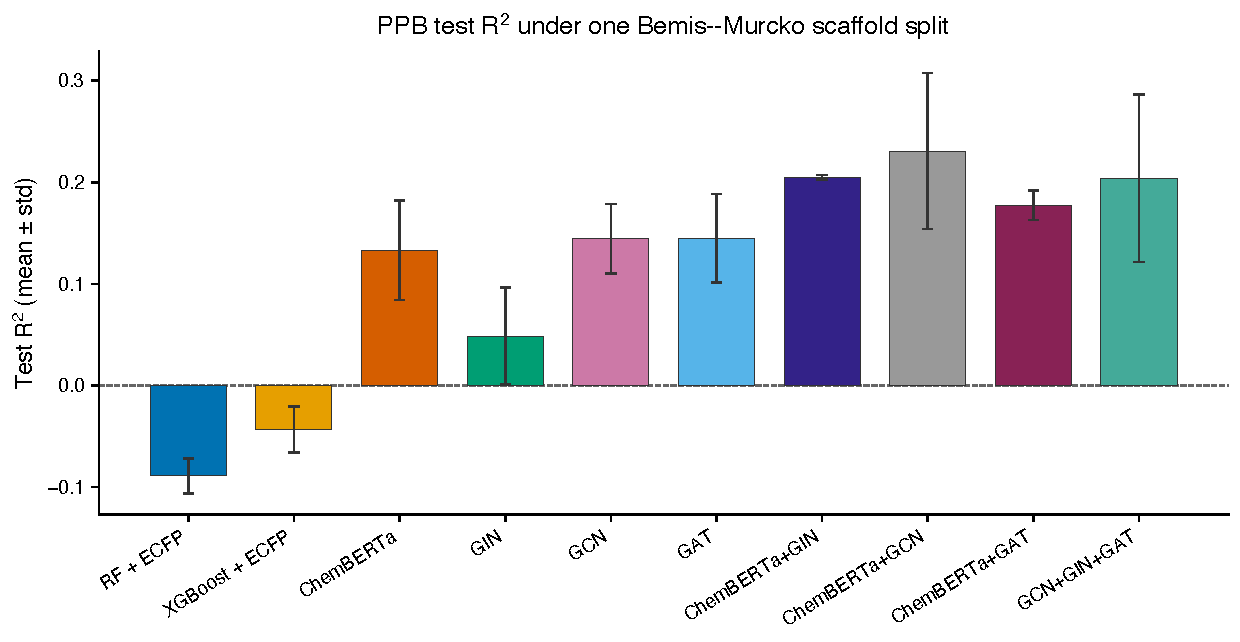
\includegraphics[width=0.95\textwidth]{fig1_test_r2_bars.pdf}
\caption{PPB test $R^{2}$ (mean $\pm$ std) under one Bemis--Murcko scaffold split. Error bars are the sample standard deviation across seeds 42, 43, and 44. Colors follow a soft Okabe--Ito palette.}
\label{fig:bars}
\end{figure}

\begin{figure}[H]
\centering
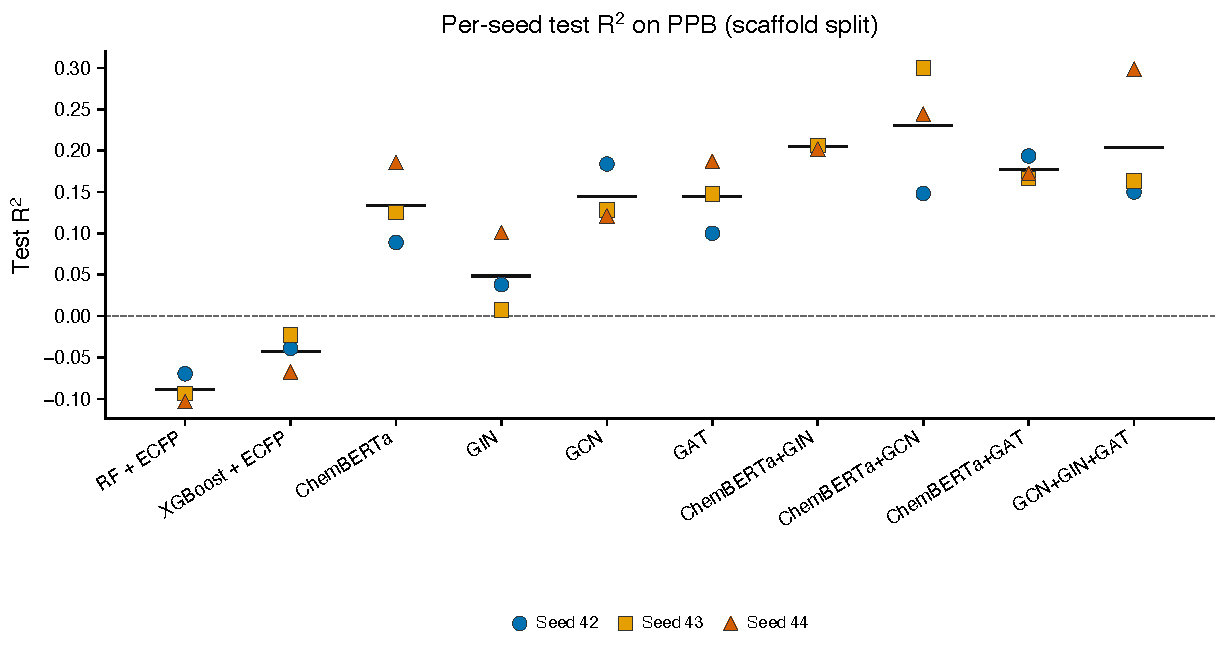
\includegraphics[width=0.95\textwidth]{fig3_seed_r2.pdf}
\caption{Per-seed PPB test $R^{2}$ on the same scaffold split. Horizontal bars mark the three-seed mean. ChemBERTa+GIN is tight across seeds; ChemBERTa+GCN and GCN+GIN+GAT are not.}
\label{fig:seeds}
\end{figure}

\subsection{Random-split control (random forest)}
Random splitting of the Random Forest (RF) model into training, validation, and testing groups improved the $R^{2}$ and the RMSE relative to Bemis--Murcko scaffold splitting.
The RF test $R^{2}$ value goes from $-0.089 \pm 0.017$ under scaffold splitting to $0.255 \pm 0.010$ under random splitting, with $\Delta R^{2} \approx 0.34$ (Table~\ref{tab:random}).
Hence, the high score of a model under random splitting should be evaluated with caution, as the model will not be able to transfer the learning to a set of molecules with an unseen core.

The splitting test is only completed for the RF model to demonstrate the effect of random vs scaffold splitting.
The random splitting is not completed for other models.
We do not expect any consistent trend because the molecules are not being separated by their scaffold structure.
The $R^{2}$ value on the testing set could increase or decrease depending on whether the model has seen the same core in the training set.
That dependency decreases the reliability of the model on unseen data.

\begin{table}[H]
\centering
\caption{Random forest + ECFP test $R^{2}$ (mean $\pm$ sample std over seeds 42--44) under DeepChem random versus scaffold splits. Seeds change the forest only; each splitter uses one molecule assignment.}
\label{tab:random}
\begin{tabular}{lcc}
\toprule
\textbf{Split} & \textbf{Test $R^{2}$} & \textbf{RMSE (\% bound)} \\
\midrule
Scaffold & $-0.089 \pm 0.017$ & $16.83 \pm 0.13$ \\
Random & $0.255 \pm 0.010$ & $12.61 \pm 0.09$ \\
\bottomrule
\end{tabular}
\end{table}

\subsection{Generalization gap and training dynamics}
None of the models transferred their learning from the training set to the testing set without a large drop in $R^{2}$.
Especially, the tree models and ChemBERTa-containing models were the worst performers in terms of overfitting.
Figure~\ref{fig:gap} demonstrates the correlation between the training $R^{2}$ and testing $R^{2}$, where each point is a seed color-coded by the model type.
All the points are well under the diagonal, suggesting none of the high scores in the training set translated to the testing set.

All the graph models sit on the left side of Figure~\ref{fig:gap}, with a smaller delta between the training and testing $R^{2}$ scores.
The individual graph models were stopped early during the training process if the model did not improve the score on the validation set for 25 epochs continuously (patience = 25).
All the ChemBERTa models were trained on a fixed schedule of 20 epochs.
That schedule allowed overfitting, and Figure~\ref{fig:gap} is consistent with that pattern.
Figure~\ref{fig:loss} demonstrates the training loss curve (epoch vs loss) for the ChemBERTa and graph models for all the seeds.

When compared to the random forest baseline, all the neural models improved the mean $R^{2}$ score on the testing set (Figure~\ref{fig:delta}).

\begin{figure}[H]
\centering
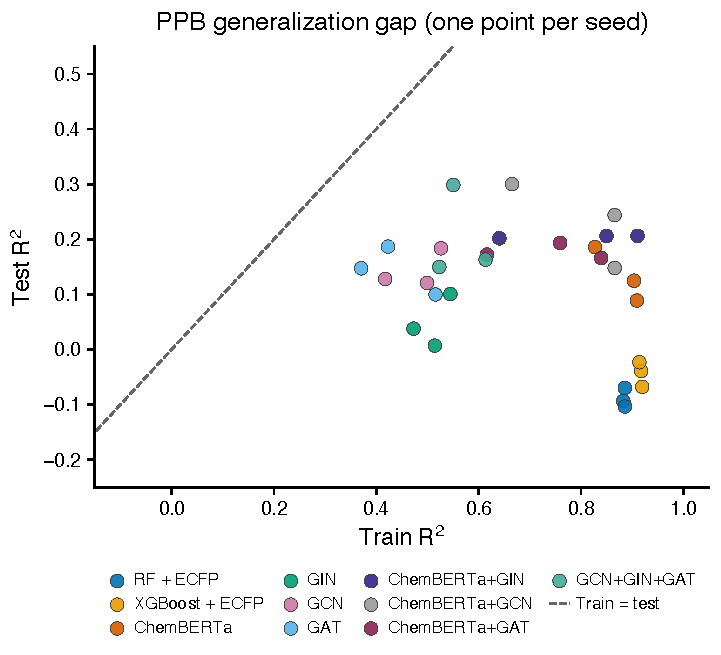
\includegraphics[width=0.62\textwidth]{fig4_generalization_gap.pdf}
\caption{Training $R^{2}$ versus test $R^{2}$ on PPB (each point is one seed). The dashed line is train $=$ test.}
\label{fig:gap}
\end{figure}

\begin{figure}[H]
\centering
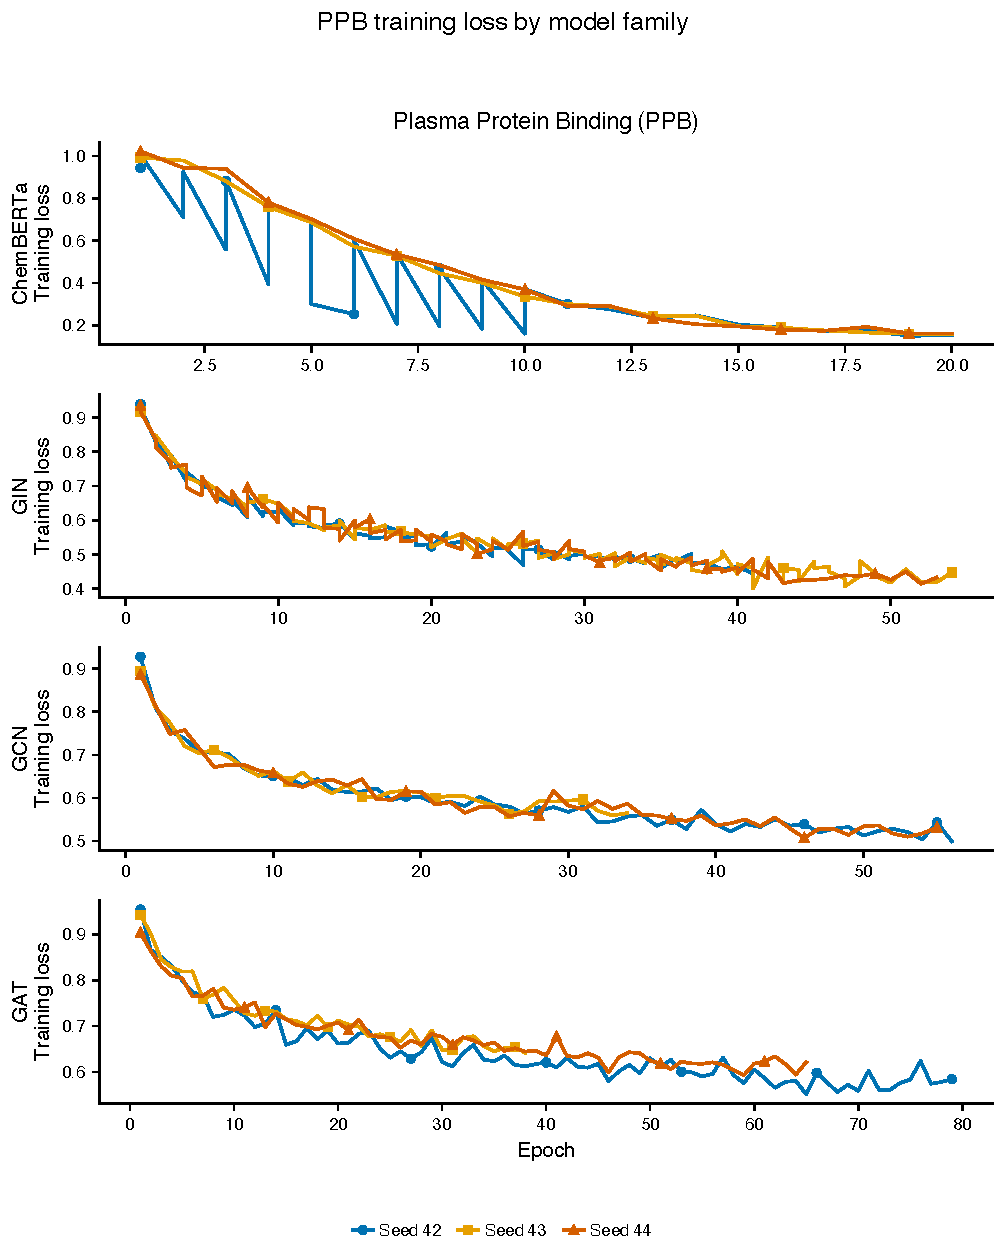
\includegraphics[width=0.82\textwidth]{fig5_loss_curves_all.pdf}
\caption{PPB training loss over epochs for ChemBERTa, GIN, GCN, and GAT. Lines are individual random seeds.}
\label{fig:loss}
\end{figure}

\begin{figure}[H]
\centering
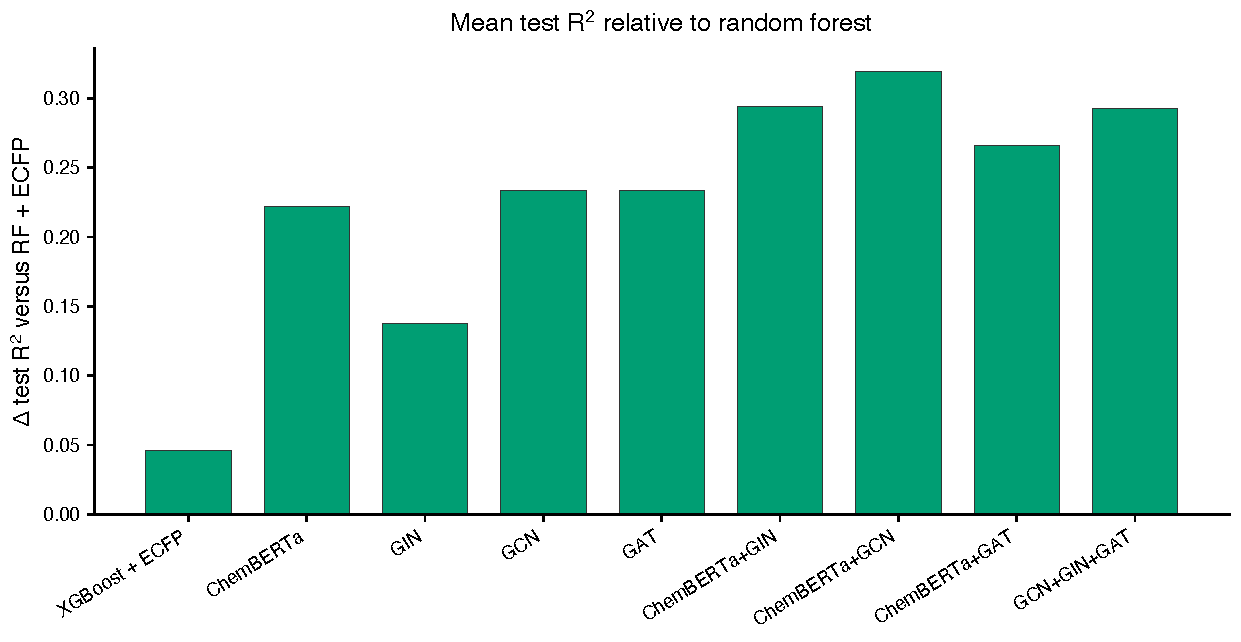
\includegraphics[width=0.95\textwidth]{fig7_delta_vs_rf.pdf}
\caption{Mean PPB test $R^{2}$ relative to random forest + ECFP under the fixed scaffold protocol.}
\label{fig:delta}
\end{figure}

\section{Discussion}

On the PPB dataset, among all the tested models, the fusion model ChemBERTa+GIN demonstrated the most stable high performance, with the lowest seed-to-seed standard deviation.
Both tree models, RF and XGBoost, failed to generalize on the testing dataset, with a negative $R^{2}$ value under scaffold split.
Scaffold splitting groups the molecules based on their core structures, and circular fingerprints capture bond patterns within a fixed radius.
The training and testing sets do not share the same core structures, which explains why the learning from the training set did not transfer to the testing set.
This idea is further supported by the control experiment with the RF model, between scaffold and random splitting, where random splitting improved the $R^{2}$ value.
As expected, random splitting places molecules with the same core into different datasets, so whenever the model came across a molecule with a similar core that it had already seen in the training sample, it was able to predict better.

GCN, GAT and ChemBERTa alone performed better than the RF and XGBoost.
Pre-trained transformers (ChemBERTa) and the graph models, including the fusion models, generalized the molecules at a more abstract level.
Hence, they managed to transfer more of the learned representation of a molecule.
They performed better on the testing group, even if they were encountering that scaffold core for the first time.
These rankings should only be interpreted qualitatively, not numerically.
Surprisingly, the GIN model alone was not able to perform comparatively to the GCN and GAT models.

The fusion models were able to learn the structure and property of a molecule better than their individual counterparts and hence exhibited a better $R^{2}$ value.
Although the performance improvement could be attributed to the increased number of parameters, that increase in the number of parameters is not large.
For example, ChemBERTa alone was $\sim$44.1 M vs ChemBERTa+GNN $\sim$44.5 M; the difference is only a small number of parameters.
Table~\ref{tab:params} presents the approximate parameter counts for each neural model, including the fusion models.
Thus, the performance improvement in the fusion models, when compared to their individual counterparts, could be a result of the models learning different chemical properties through the different architectures.

The marginal improvement of the ChemBERTa+GAT model in comparison to its individual models could be attributed to the lack of diversity in the model architecture.
ChemBERTa is a transformer-based model with attention over SMILES tokens and GAT is a graph network with attention over graph neighbors, but both still used an attention mechanism to understand the molecules.
Hence, they may have fallen behind in rationalizing the molecular semantics.
When we bring a different kind of model to the fusion, it understands molecules from a different perspective.

\section{Conclusions}

For the PPB dataset, a graph network in combination with other graph networks or a transformer model such as ChemBERTa performed better than just a graph network or ChemBERTa itself.
Fusion models with variable architectures learned different structure-property relationships that individual models could not.
Scaffold splitting provides a much stricter split and better evaluates whether a model can transfer the understanding of a molecule to a future unseen group of molecules that do not share the same core.
Performance of a model that is trained on a randomly split dataset should not be overemphasized during benchmarking, as the performance improvement could simply be an artifact of luck and randomness.
Even if the $R^{2}$ value may not be large, a much better approach for a benchmarking procedure is scaffold splitting, because the model could be more applicable to truly new unseen data.
Future studies will explore whether this performance improvement of the fusion model translates to other publicly available datasets.

\section*{Data and code}
The PPB dataset was accessed through DeepChem's MoleculeNet~\cite{wu2018moleculenet} with z-score normalization fit on the training set.
Training and evaluation scripts, environment freeze files, figures, model leaderboards, and supplementary files will be available at \url{https://github.com/kcncell/PPB\_benchmark\_GNN\_chemBERTa} when the ChemRxiv preprint goes public.

\section*{Author contributions}
Pradyumna Kumar Pradhan (Independent Researcher; previously Professional Track Faculty at UNC Greensboro) designed and implemented this project, analyzed the results, and wrote the manuscript.
AI was used only to correct grammar and typos and to help with the code.

\section*{Competing interests}
The author declares no competing interests.

\section*{Acknowledgements}
This work used DeepChem, PyTorch, PyTorch Geometric, Hugging Face Transformers, RDKit, scikit-learn, XGBoost, and related open-source tools on an Apple M1 Mac Mini.
AI was used only to correct grammar and typos and to help with the code.
All scientific content, experimental design, results, and conclusions were conceived, executed, and verified by the author.
No external funding supported the study.

\begin{thebibliography}{99}

\bibitem{bohnert2013ppb}
Bohnert T, Gan LS.\ (2013)
Plasma protein binding: from discovery to development.
\emph{Journal of Pharmaceutical Sciences} 102:2953-2994.
doi:10.1002/jps.23614.

\bibitem{sun2018ppb}
Sun L, Yang H, Li J, Wang T, Li W, Liu G, Tang Y.\ (2018)
In silico prediction of compounds binding to human plasma proteins by QSAR models.
\emph{ChemMedChem} 13:572-581.
doi:10.1002/cmdc.201700582.

\bibitem{ghafourian2013ppb}
Ghafourian T, Amin Z.\ (2013)
QSAR models for the prediction of plasma protein binding.
\emph{BioImpacts} 3:21-27.
doi:10.5681/bi.2013.011.

\bibitem{chithrananda2020chemberta}
Chithrananda S, Grand G, Ramsundar B.\ (2020)
ChemBERTa: large-scale self-supervised pretraining for molecular property prediction.
arXiv:2010.09885.

\bibitem{yang2019analyzing}
Yang K, Swanson K, Jin W, Coley C, Eiden P, Gao H, Guzman-Perez A, Hopper T, Kelley B, Mathea M, Palmer A, Settels V, Jaakkola T, Jensen K, Barzilay R.\ (2019)
Analyzing learned molecular representations for property prediction.
\emph{Journal of Chemical Information and Modeling} 59:3370-3388.
doi:10.1021/acs.jcim.9b00237.

\bibitem{fabian2020molbert}
Fabian B, Edlich T, Gaspar H, Segler M, Meyers J, Fiscato M, Ahmed M.\ (2020)
Molecular representation learning with language models and domain-relevant auxiliary tasks.
arXiv:2011.13230.

\bibitem{ahmad2022chemberta2}
Ahmad W, Simon E, Chithrananda S, Grand G, Ramsundar B.\ (2022)
ChemBERTa-2: towards chemical foundation models.
arXiv:2209.01712.

\bibitem{sheridan2013time}
Sheridan RP.\ (2013)
Time-split cross-validation as a method for estimating the goodness of prospective prediction.
\emph{Journal of Chemical Information and Modeling} 53:783-790.
doi:10.1021/ci400084k.

\bibitem{wu2018moleculenet}
Wu Z, Ramsundar B, Feinberg EN, Gomes J, Geniesse C, Pappu AS, Leswing K, Pande V.\ (2018)
MoleculeNet: a benchmark for molecular machine learning.
\emph{Chemical Science} 9:513-530.
doi:10.1039/C7SC02664A.

\bibitem{ramsundar2019deep}
Ramsundar B, Eastman P, Walters P, Pande V.\ (2019)
\emph{Deep Learning for the Life Sciences}.
Sebastopol, CA: O'Reilly Media.

\bibitem{bemis1996scaffold}
Bemis GW, Murcko MA.\ (1996)
The properties of known drugs. 1.\ Molecular frameworks.
\emph{Journal of Medicinal Chemistry} 39:2887-2893.
doi:10.1021/jm9602928.

\bibitem{rogers2010ecfp}
Rogers D, Hahn M.\ (2010)
Extended-connectivity fingerprints.
\emph{Journal of Chemical Information and Modeling} 50:742-754.
doi:10.1021/ci100050t.

\bibitem{gilmer2017mpnn}
Gilmer J, Schoenholz SS, Riley PF, Vinyals O, Dahl GE.\ (2017)
Neural message passing for quantum chemistry.
In: \emph{Proceedings of the 34th International Conference on Machine Learning (ICML)}, PMLR 70:1263-1272.

\bibitem{kipf2017gcn}
Kipf TN, Welling M.\ (2017)
Semi-supervised classification with graph convolutional networks.
In: \emph{International Conference on Learning Representations (ICLR)}.

\bibitem{xu2019gin}
Xu K, Hu W, Leskovec J, Jegelka S.\ (2019)
How powerful are graph neural networks?
In: \emph{International Conference on Learning Representations (ICLR)}.

\bibitem{velickovic2018gat}
Veli{\v{c}}kovi{\'c} P, Cucurull G, Casanova A, Romero A, Li{\`o} P, Bengio Y.\ (2018)
Graph attention networks.
In: \emph{International Conference on Learning Representations (ICLR)}.

\bibitem{xiong2020attentivefp}
Xiong Z, Wang D, Liu X, Zhong F, Wan X, Li X, Li Z, Luo X, Chen K, Jiang H, Zheng M.\ (2020)
Pushing the boundaries of molecular representation for drug discovery with the graph attention mechanism.
\emph{Journal of Medicinal Chemistry} 63:8749-8760.
doi:10.1021/acs.jmedchem.9b00959.

\bibitem{rollins2024molprop}
Rollins ZA, Cheng AC, Metwally E.\ (2024)
MolPROP: molecular property prediction with multimodal language and graph fusion.
\emph{Journal of Cheminformatics} 16:56.
doi:10.1186/s13321-024-00846-9.

\bibitem{vovk2005algorithmic}
Vovk V, Gammerman A, Shafer G.\ (2005)
\emph{Algorithmic Learning in a Random World}.
New York: Springer.

\bibitem{angelopoulos2021gentle}
Angelopoulos AN, Bates S.\ (2021)
A gentle introduction to conformal prediction and distribution-free uncertainty quantification.
arXiv:2107.07511.

\bibitem{svensson2018conformal}
Svensson F, Aniceto N, Norinder U, Cortes-Ciriano I, Spjuth O, Carlsson L, Bender A.\ (2018)
Conformal regression for quantitative structure-activity relationship modeling: quantifying prediction uncertainty.
\emph{Journal of Chemical Information and Modeling} 58:1132-1140.
doi:10.1021/acs.jcim.8b00054.

\end{thebibliography}


\end{document}
